\section{Motivation}

\begin{frame}
\frametitle{Direct Numerical Simulation}
\pause
\begin{columns}
\begin{column}{0.5\textwidth}
\begin{itemize}
    \item<2-> DNS: approach for solving
        the Navier-Stokes equations
    \item<3-> Aim: resolve all the spatial and temporal
        features of the flow
    \item<4-> Use a fine computational grid
        to represent the flow domain;
        some numerical method to solve N-S equations
    \item<7-> Popular numerical methods:
        \begin{itemize}
            \item<8-> \alert<11> {finite difference methods}
            \item<9-> spectral methods
            \item<10-> finite element methods
        \end{itemize}
\end{itemize}
\end{column}
\begin{column}{0.5\textwidth}
\vspace{1.5cm}
\hspace{1cm}
\includegraphics<4>[width=100px]
    {img/simple-flow-domain.eps}
\includegraphics<5>[width=100px]
    {img/simple-grid.eps}   
\includegraphics<6->[width=100px]
    {img/simple-flow-solution.eps}   
\end{column}
\end{columns}
\end{frame}

\begin{frame}[t]
\frametitle{DNS: an expensive endaevour}
\pause
\begin{columns}[T]
\begin{column}{0.5\textwidth}
\begin{itemize}[<+->]
    \item Requires very fine grids,
        and expensive numerical schemes
        \begin{itemize}[<+->]
            \item impractical except for simple flows
            \item parallel solution almost always required
        \end{itemize}
    \item Traditional workhorse for computation: CPU core
    \item Algorithms exhibit fine-grained parallelism
        \begin{itemize}[<+->]
            \item Pointwise computations
            \item Stencil computations
        \end{itemize}
    \item Well suited to graphics processing units (GPUs)
\end{itemize}
\end{column}
\begin{column}{0.5\textwidth}
    \centering
    \only<4> {\includegraphics[height=175px]{img/tasks.eps}}
    \only<5-6> {\includegraphics[height=175px]{img/cpu-tasks.eps}}
    \only<7> {\includegraphics[height=175px]{img/pointwise.eps}}
    \only<8> {\includegraphics[height=175px]{img/pointwise-stencil.eps}}
    \only<9> {\includegraphics[height=175px]{img/gpu-tasks.eps}}
\end{column}
\end{columns}
\end{frame}

\begin{frame}
\frametitle{Compact finite difference schemes}
\pause
\begin{columns}
\begin{column}{0.5\textwidth}
\begin{itemize}[<+->]
    \item A class of high-order accurate finite difference schemes
        for evaluating spatial derivatives
    \item Much better at resolving high wavenumbers compared
        to explicit schemes
    \item Require less communication between parallel processes
\end{itemize}
\end{column}
\begin{column}{0.5\textwidth}
    \visible<3->{\includegraphics[width=180px]{img/modified-wavenumbers.eps}}
\end{column}
\end{columns}
\end{frame}

\begin{frame}
\frametitle{Compact finite difference schemes}
\begin{alert}{Comes at a cost!}
\pause
\begin{itemize}[<+->]
    \item Requires solution of \emph{banded} linear systems
    \item Simplest case: tridiagonal systems
    \item More expensive to evaluate than explicit schemes
    \item Difficult to parallelize
        \begin{itemize}[<+->]
            \item Classical \emph{Thomas algorithm} exhibits
                neither coarse-grained nor fine-grained parallelism
        \end{itemize}
\end{itemize}
\end{alert}
\end{frame}

\begin{frame}
\frametitle{Objectives}
\begin{itemize}
    \item Exploratory work for exploiting GPUs
        in current research code
        \begin{itemize}
            \item important step for our group: Palmetto cluster
        currently has 598 GPUs (and counting)
        \end{itemize}
    \item An efficient GPU tridiagonal solver
    \item Parallelize the compact finite difference evaluation---current
        research code uses a sequential approach
\end{itemize}
\end{frame}

\begin{frame}
\frametitle{Thesis contributions}
\begin{itemize}
    \item A novel solution strategy for
        the tridiagonal systems arising in
        compact finite differences
        and other numerical schemes
    \item A strategy for evaluating compact
        finite differences on GPU-accelerated clusters
\end{itemize}
\end{frame}
